\documentclass[11pt]{article}
\usepackage{fullpage}
\usepackage{graphics,epsfig,color}
\usepackage{wrapfig}
\usepackage{amsmath}
\usepackage{forest}
\usepackage{times}
\usepackage{setspace}
\usepackage{amsmath,amsthm,amssymb}
\usepackage{subfigure}
\usepackage{url}
\newtheorem{problem}{Problem}
\newtheorem{answer}{Answer}
\usepackage{listings}
\usepackage{color}
\usepackage{adjustbox}
\usepackage{tikz}
\definecolor{dkgreen}{rgb}{0,0.6,0}
\definecolor{gray}{rgb}{0.5,0.5,0.5}
\definecolor{mauve}{rgb}{0.58,0,0.82}
\usepackage{graphicx}
\graphicspath{ {images/} }

\lstset{frame=tb,
	language=Java,
	aboveskip=3mm,
	belowskip=3mm,
	showstringspaces=false,
	columns=flexible,
	basicstyle={\small\ttfamily},
	numbers=none,
	numberstyle=\tiny\color{gray},
	keywordstyle=\color{blue},
	commentstyle=\color{dkgreen},
	breaklines=true,
	breakatwhitespace=true,
	tabsize=3
}

\begin{document}
\begin{center}
	{\LARGE CSCD320 Homework7}
	
	\bigskip
	
	{\Large Ethan Tuning}
\end{center}

\bigskip

\begin{problem}
 \label{prob:1}
 Show a minimum spanning tree of the following connected undirected graph by using any method. You don't have to trace the algorithm that you use, but instead you can just show the MST by making the tree edges in different color.
\begin{center}
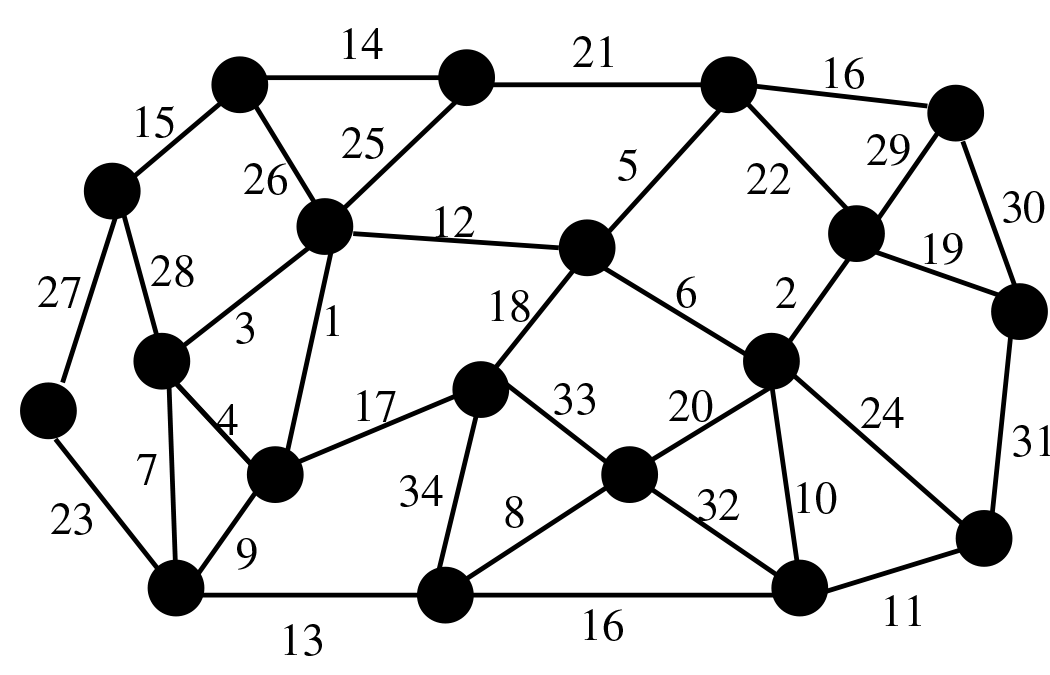
\includegraphics[width=4cm, height=3cm]{graph1}
\end{center}
\end{problem}

\begin{answer}
 \label{ans:1}
 Here is the answer.
\begin{center}
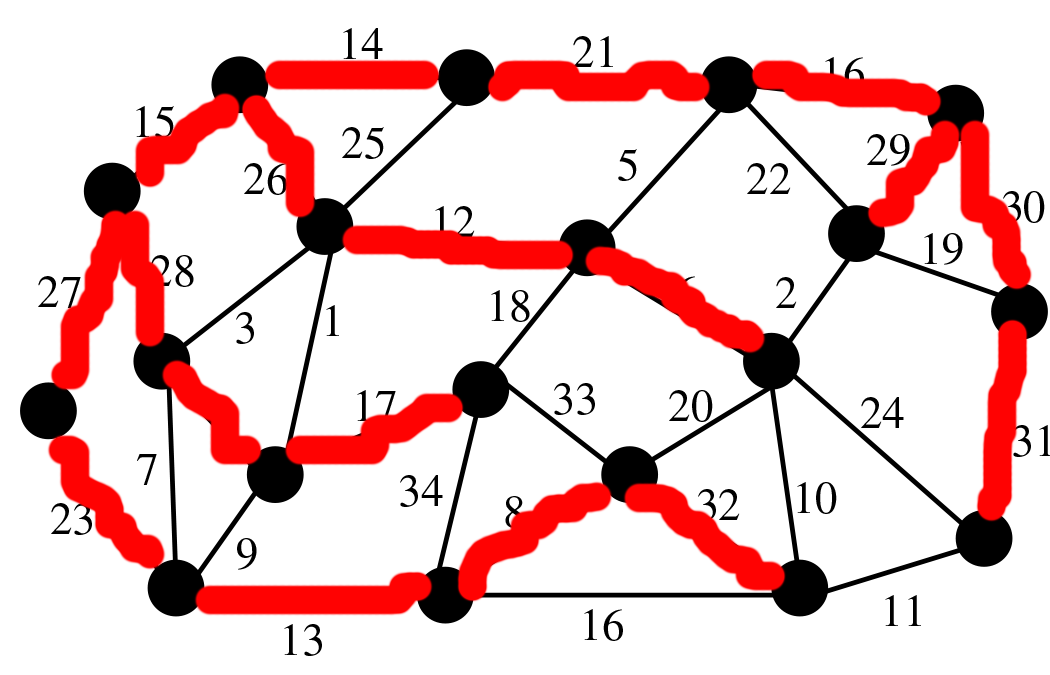
\includegraphics[width=4cm, height=3cm]{graph2}
\end{center}
\end{answer}

\bigskip

\begin{problem}
 \label{prob:2}
 Trace the Dijastra's algorithm to show the shortest paths from the vertex s to all the other vertices in the following connected directed graph.
\begin{center}
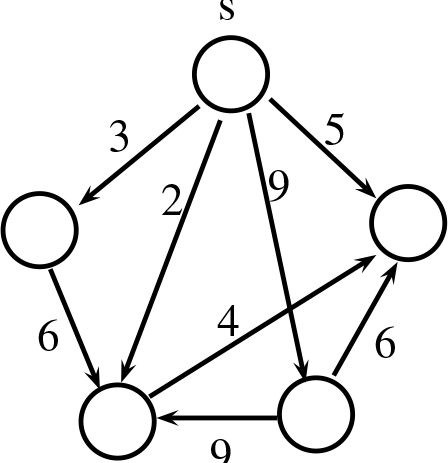
\includegraphics[width=3cm, height=3cm]{graph3}
\end{center}
\end{problem}

\begin{answer}
 \label{ans:2}
 Here is the answer.
\begin{center}
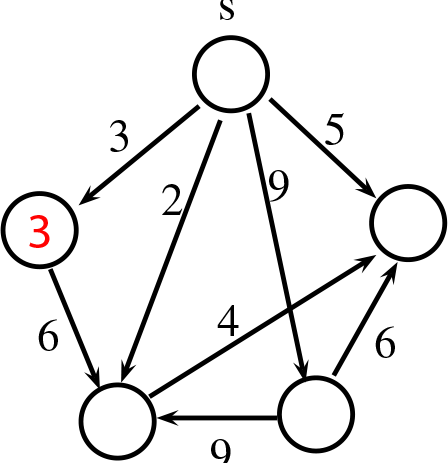
\includegraphics[width=3cm, height=3cm]{dgraph1}
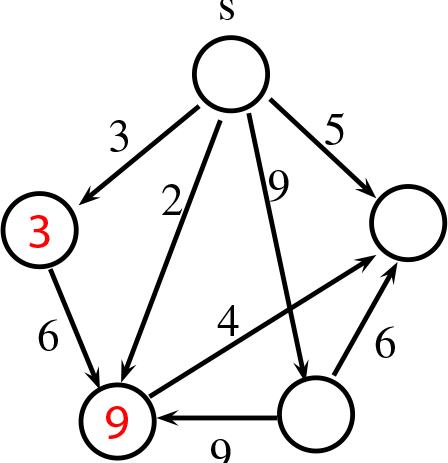
\includegraphics[width=3cm, height=3cm]{dgraph2}
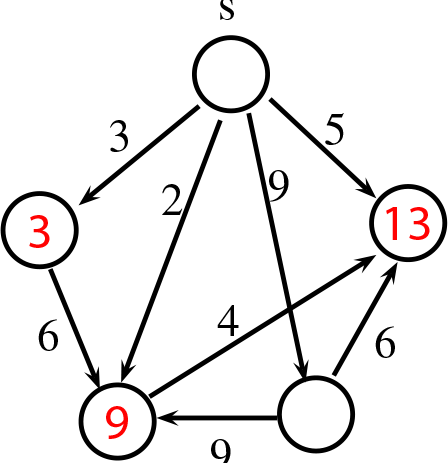
\includegraphics[width=3cm, height=3cm]{dgraph3}
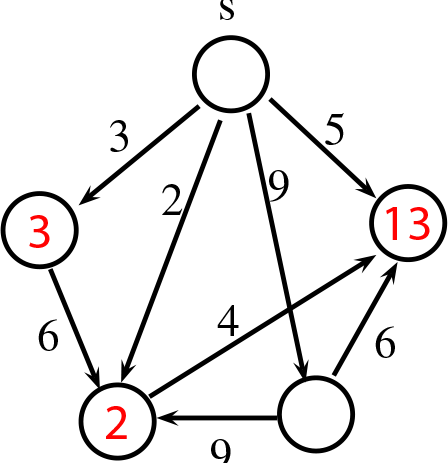
\includegraphics[width=3cm, height=3cm]{dgraph4}
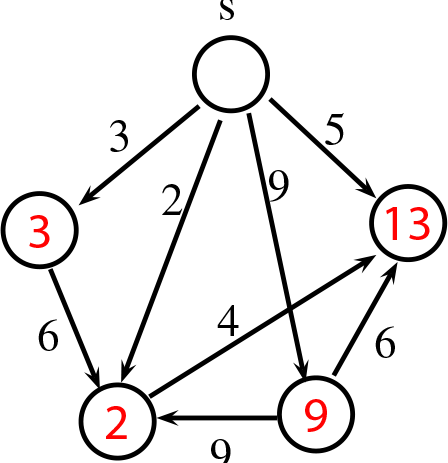
\includegraphics[width=3cm, height=3cm]{dgraph5}
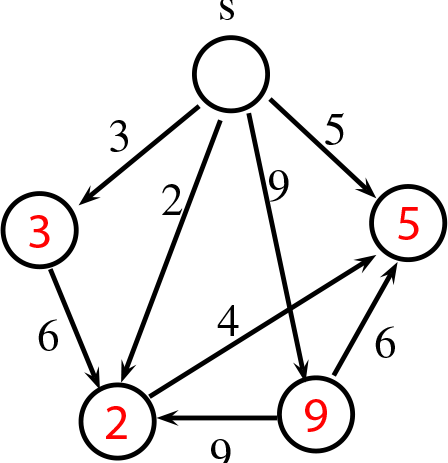
\includegraphics[width=3cm, height=3cm]{dgraph6}
\end{center}
\end{answer}

\bigskip

\begin{problem}
 \label{prob:3}
 Give an $O(|V|*|E|)$ time algorithm for computing the transitive closure of a directed graph $G = (V,E)$. You can assume $|E| \geq |V|$.
\end{problem}

\begin{answer}
 \label{ans:3}
 Here is some peusdocode.
\begin{lstlisting}
for (int v = 0; v < G.V; v++)
	DFS(G, v);
\end{lstlisting}
\end{answer}

\bigskip

\begin{problem}
 \label{prob:4}
 The Floyd-Warshall algorithm uses the matrix $D^0$ to find the all-pair shortest
 paths. That is, it uses $D^0$ to calculate the matrices $D^1,D^2,D^3, . . .,D^n,$ where each entry $(d^n)_ij$ in $D^n$ is the shortest distance from i to $j$, for every $i$ and $j, 1 \leq i, j \leq n$. Given the following example $D^0$, calcualte $D^1, D^2, D^3, and D^4$. You don’t have to show the details of the calculation, instead you can just show the content of each matrix of $D^1, D^2, D^3, and D^4$.
 
\begin{center}
\[
D^0=
\begin{bmatrix}
0 & 5 & \infty & 3 \\
\infty & 0 & -1 & \infty \\
6 & \infty & 0 & \infty \\
\infty & 2 & 7 & 0
\end{bmatrix}
\]
\end{center}
\end{problem}

\begin{answer}
 \label{ans:4}
 Here is the answer.
\begin{center}
\[
D^1=
\begin{bmatrix}
0 & 5 & \infty & 3 \\
4 & 0 & -1 & \infty \\
6 & \infty & 0 & \infty \\
\infty & 2 & 7 & 0
\end{bmatrix}

\bigskip

D^2=
\begin{bmatrix}
0 & 5 & \infty & 3 \\
4 & 0 & -1 & \infty \\
6 & \infty & 0 & \infty \\
7 & 2 & 7 & 0
\end{bmatrix}

\bigskip

D^3=
\begin{bmatrix}
0 & 5 & \infty & 3 \\
4 & 0 & -1 & \infty \\
6 & 5 & 0 & \infty \\
7 & 2 & 7 & 0
\end{bmatrix}

\bigskip

D^4=
\begin{bmatrix}
0 & 5 & 4 & 3 \\
4 & 0 & -1 & \infty \\
6 & 5 & 0 & \infty \\
7 & 2 & 7 & 0
\end{bmatrix}
\]
\end{center}
\end{answer}
\end{document}